\documentclass[]{article}
\usepackage{amsmath}
\usepackage{graphicx}
\graphicspath{.}

%opening
\title{AERO 7970 - Multivariable Control of Uncertain Systems \\ Homework 1}
\author{Matt Boler}

\begin{document}

\maketitle

\section{Assignment}
Design a control system using frequency shaping for the following system:

\begin{equation}
	G(s) = \frac{10}{(s+1)^2}
	\label{eq:G}
\end{equation}
\noindent to satisfy the performance requirements:
\begin{itemize}
	\item Steady state error to a unit step = 0
	\item -40dB attenuation in the frequency range [0.01-0.1] rad/sec
	\item -40dB attenuation in the frequency range [100-1000] rad/sec
	\item Bandwidth of approximately 10 rad/sec
	\item Phase margin of 30 degrees
\end{itemize}

\section{Solution}

\begin{figure}[h]
	\caption{Plant Response}
	\centering
	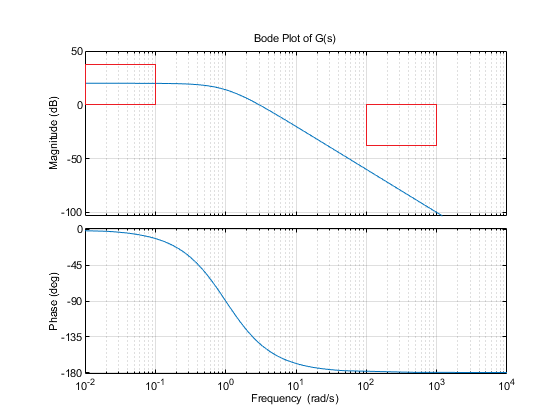
\includegraphics{Plant}
	\label{fig:plant}
\end{figure}

The loop shaping requirements and uncontrolled plant response are shown in Figure \ref{fig:plant}.
From these requirements, $\Lambda(s)$ was designed in Matlab's Bode Design Editor to satisfy the loop shaping requirements.
The frequency response of $\Lambda(s)$ is shown in Figure \ref{fig:lambda}.

\begin{align}
	\Lambda(s) &= 35.948 \frac{(s+0.1049)(s+0.1117)}{(s + 9.99)^2} \\
	W(s) = \Lambda^{-1} &= .027818 \frac{(s+9.99)^2}{(s + 0.1049)(s+0.1117)}
\end{align}



As zero steady-state error to a step input is required, it is know that the controller $K(s)$ will include a $\frac{1}{s}$ term.
By starting with this, the controller $K(s)$ was designed using Matlab's Bode Design Editor, shown in Figure \ref{fig:design}.

\begin{equation}
	K(s) = 115.74 \frac{(s+1)^2 (s+1.825) (s + 0.008682) (s^2 + 1.433s + 8583)}{s (s + 1613) (s + 21.4)^2 (s + 0.2313)^2}
	\label{eq:K}
\end{equation} 

As shown in Figures \ref{fig:sw} and \ref{fig:sens}, the loop transfer and sensitivity resulting from this controller satisfy the requirements:
\begin{align*}
	|S(s)W(s)| &\leq 1 \forall s \in \mathit{C_+} \\
	|S(s)| &\leq |\Lambda(s)| \forall s \in \mathit{C_+}
\end{align*} 

The resulting closed loop system is 

\begin{equation}
	\frac{K(s)G(s)}{1+K(s)G(s)}
\end{equation}.
Figures \ref{fig:margin} and \ref{fig:cl} show that the system fulfills the margin and closed loop response requirements.

\begin{figure}[h]
	\caption{$\Lambda$ Frequency Shaping}
	\centering
	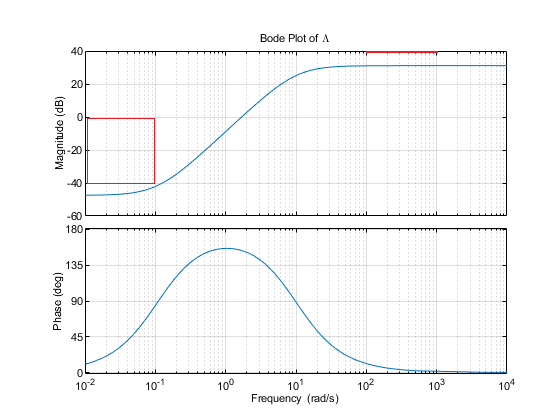
\includegraphics[width=\textwidth]{Lambda}
	\label{fig:lambda}
\end{figure}

\begin{figure}[h]
	\caption{$K(s)$ Frequency Shaping}
	\centering
	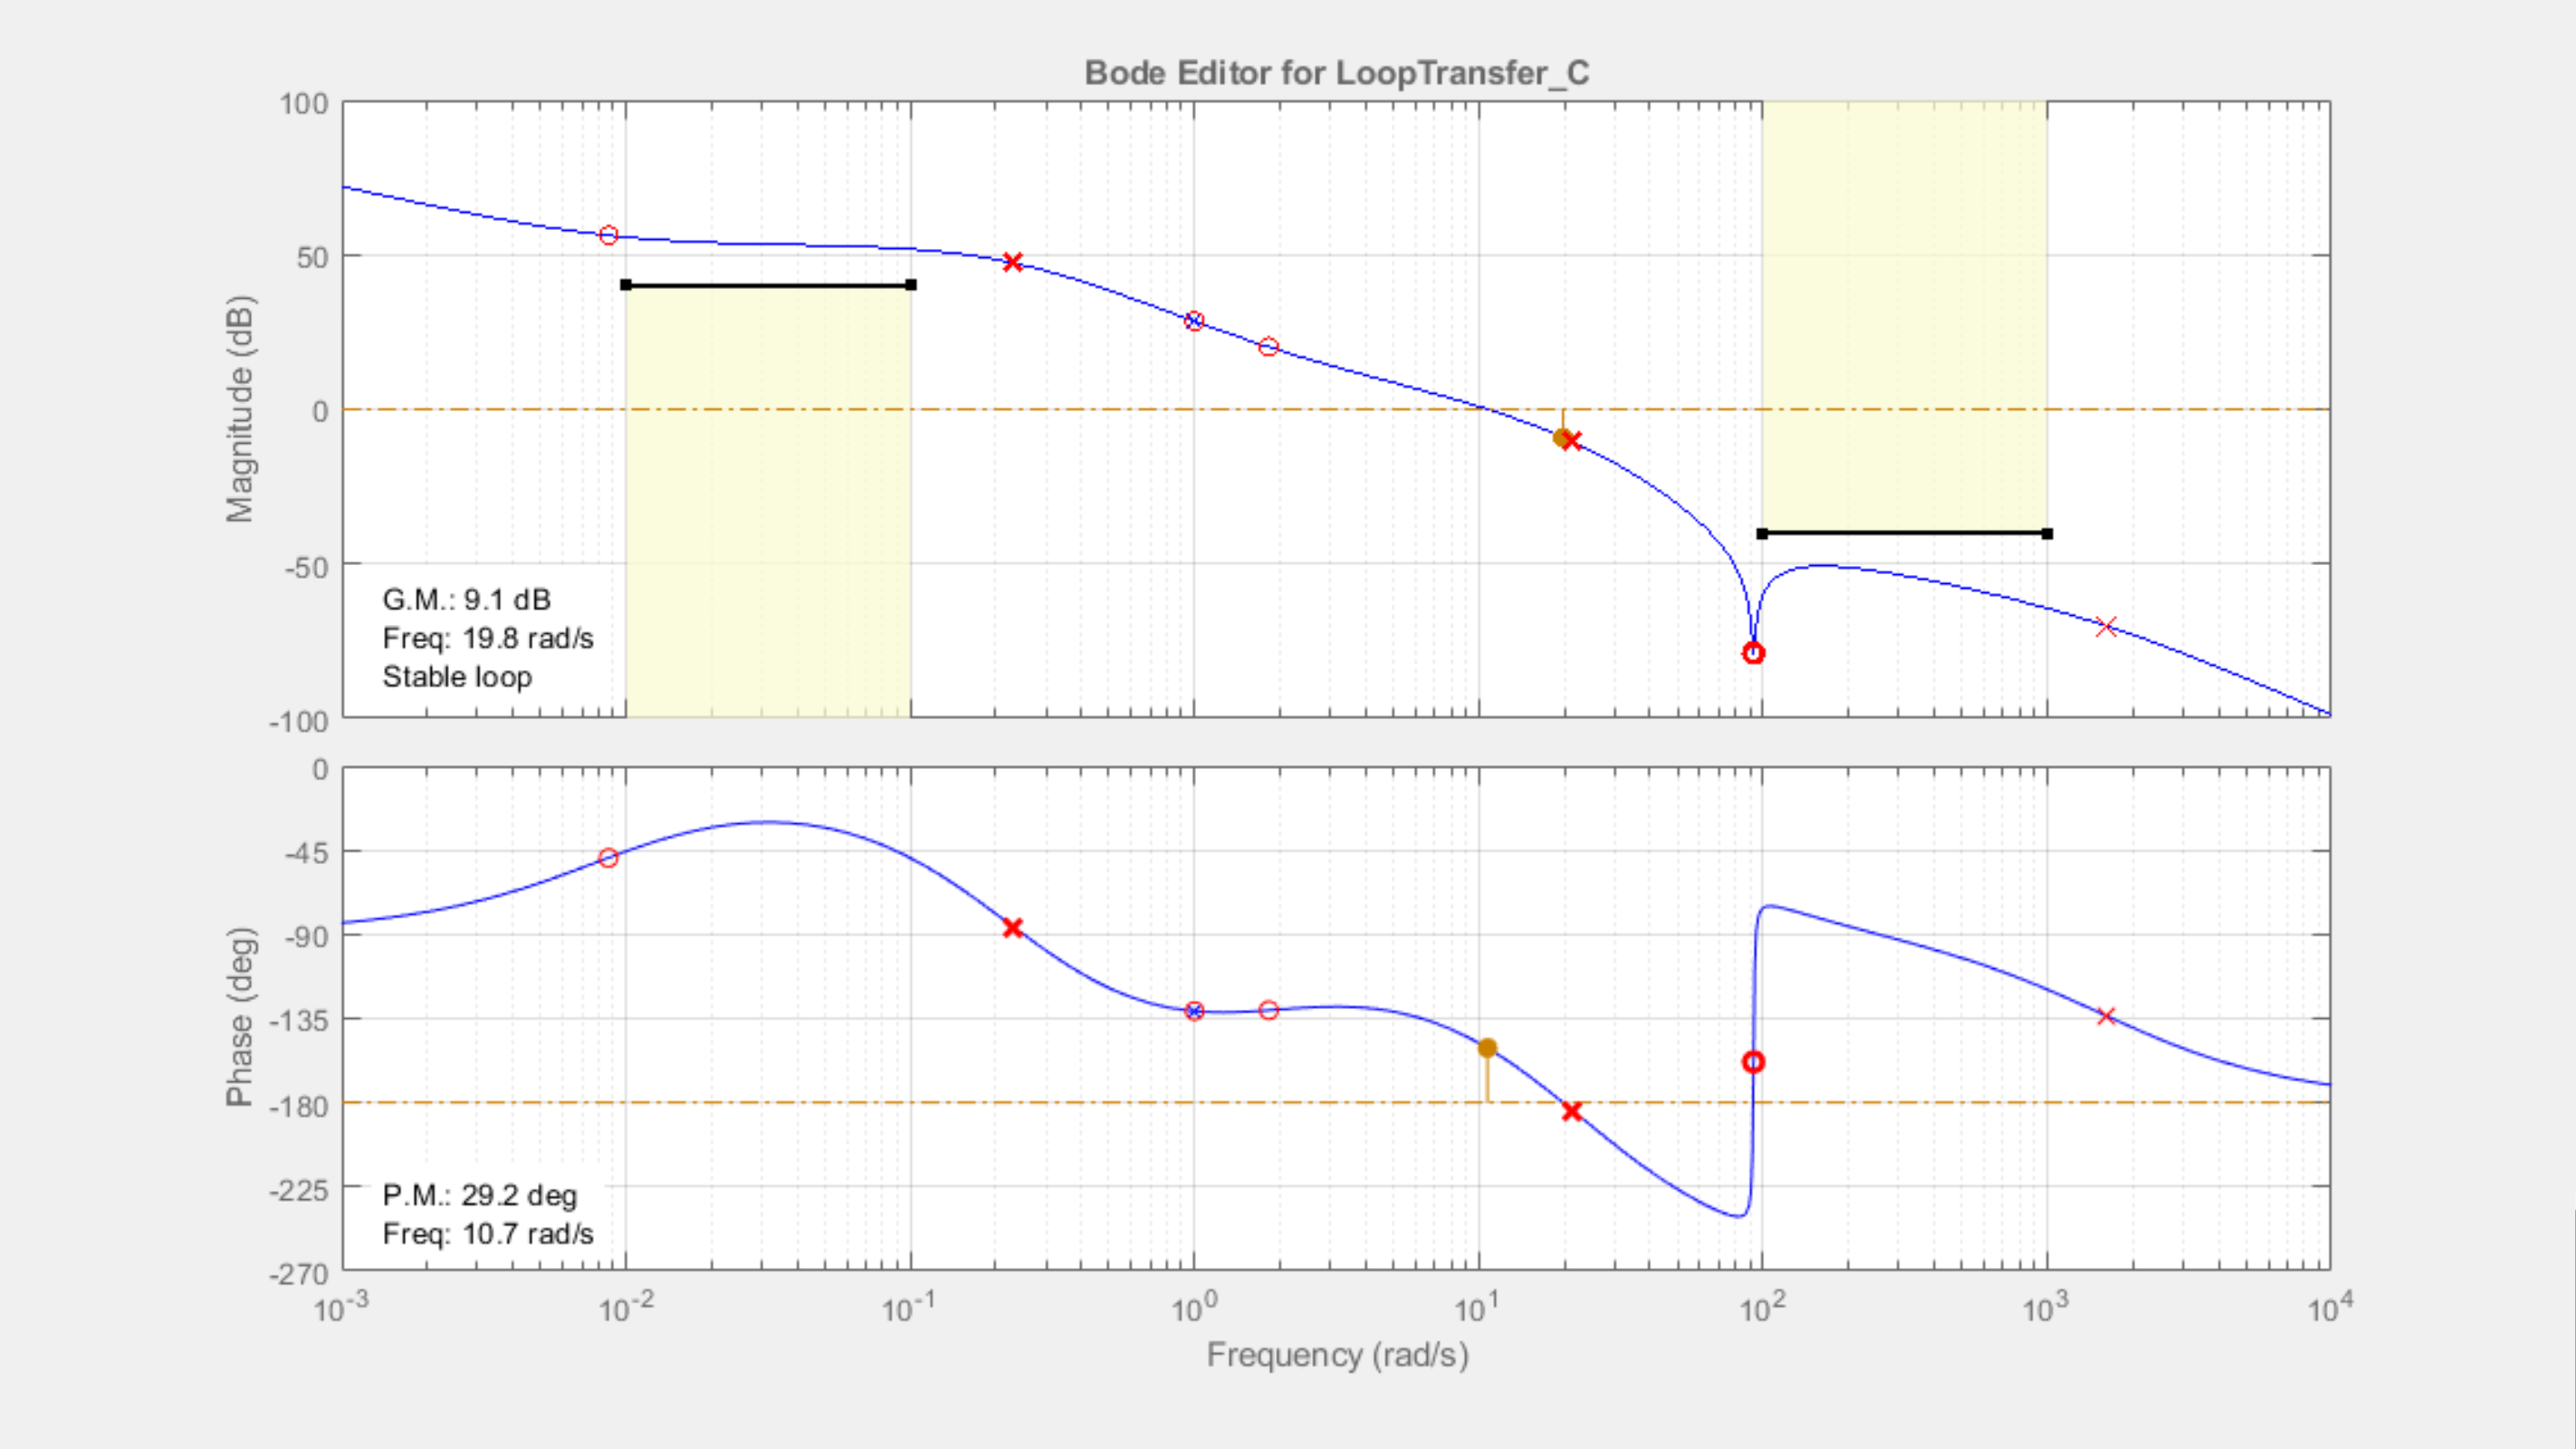
\includegraphics[width=\textwidth]{designing}
	\label{fig:design}
\end{figure}

\begin{figure}[h]
	\caption{$S(s) * W(s)$}
	\centering
	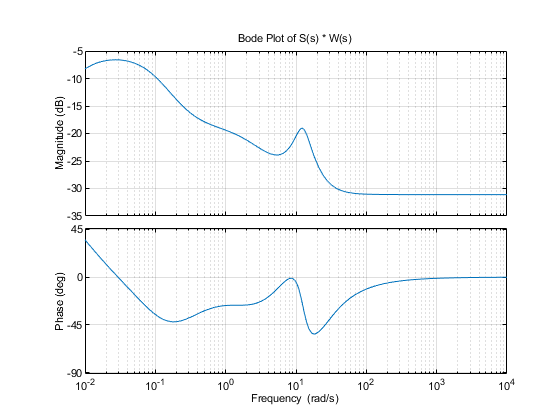
\includegraphics[width=\textwidth]{SensitivityTimesW}
	\label{fig:sw}
\end{figure}

\begin{figure}[h]
	\caption{Sensitivity vs $\Lambda$}
	\centering
	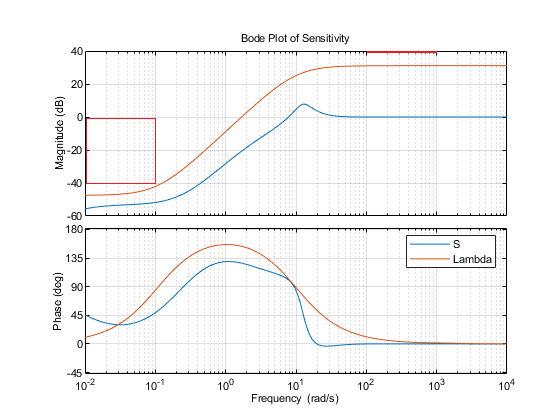
\includegraphics[width=\textwidth]{Sensitivity}
	\label{fig:sens}
\end{figure}

\begin{figure}[h]
	\caption{Stability Margins and Frequency Response}
	\centering
	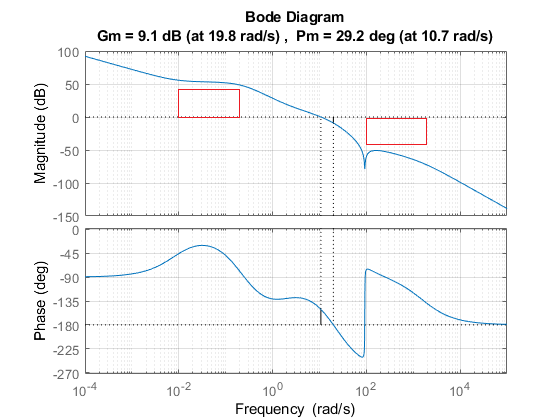
\includegraphics[width=\textwidth]{margin}
	\label{fig:margin}
\end{figure}

\begin{figure}[h]
	\caption{Closed Loop Response}
	\centering
	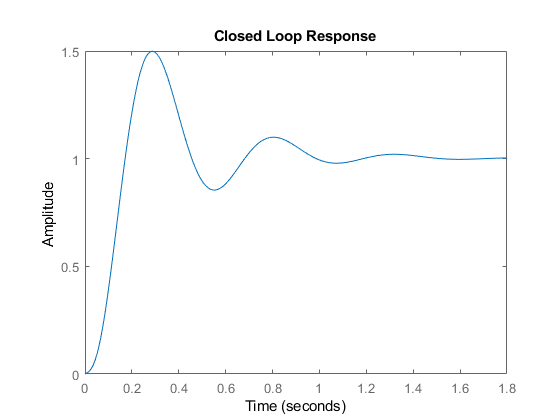
\includegraphics[width=\textwidth]{ClosedLoop}
	\label{fig:cl}
\end{figure}

\end{document}
